\documentclass{article}
\usepackage{graphicx}
\usepackage{titletoc}
\usepackage{titlesec}
\usepackage{geometry} 
\usepackage{fontspec, xunicode, xltxtra}
\usepackage{float}
\usepackage{cite}
\usepackage{amsmath}
\usepackage{listings}
\usepackage{titletoc}
\usepackage{bm}

\geometry{left=3cm,right=3cm,top=3cm,bottom=3cm}
\DeclareMathOperator*{\argmin}{argmin}
\DeclareMathOperator*{\argmax}{argmax}
\DeclareMathOperator*{\var}{var}
\DeclareMathOperator*{\expec}{E}

\begin{document}
\title{\textsf{Homework 3 for Pattern Recognition}}
\author{Fan JIN\quad (2015011506)}
\maketitle

\section*{Question 1}
{
    \[
    \begin{split}
        &   \frac{\partial}{\partial \hat{\theta}} R(\hat{\theta} | \bm{X}) \\
        =&  \frac{\partial}{\partial \hat{\theta}} \int_{\theta} {(\hat{\theta}-\theta)^2 p(\theta | \bm{X}) \mathrm{d}\theta} \\
        =&  \int_{\theta} {\frac{\partial}{\partial \hat{\theta}} (\hat{\theta}-\theta)^2 p(\theta | \bm{X}) \mathrm{d}\theta} \\
        =&  \int_{\theta} {2 (\hat{\theta}-\theta) p(\theta | \bm{X}) \mathrm{d}\theta} \\
        =&  \int_{\theta} {2 \hat{\theta} p(\theta | \bm{X}) \mathrm{d}\theta} - \int_{\theta} {2 \theta p(\theta | \bm{X}) \mathrm{d}\theta} \\
        =&  \hat{\theta} \cdot \int_{\theta} {2 p(\theta | \bm{X}) \mathrm{d}\theta} - \int_{\theta} {2 \theta p(\theta | \bm{X}) \mathrm{d}\theta} \\
        =&  \hat{\theta} \cdot 2 - \int_{\theta} {2 \theta p(\theta | \bm{X}) \mathrm{d}\theta} = 0.
    \end{split}
    \]

    The solution to the equation above is $$\hat{\theta} = \int_{\theta} {\theta p(\theta | \bm{X}) \mathrm{d}\theta}.$$

    Note that $$\frac{\partial^2}{\partial \hat{\theta}^2} R(\hat{\theta} | \bm{X}) = 2 > 0,$$ which means the solution above is the global minimum for $\hat{\theta}$. Thus, we have $$\theta^{*} = \int_{\theta} {\theta p(\theta | \bm{X}) \mathrm{d}\theta}.$$

}

\section*{Question 2}
{
    \subsection*{(1)}
    {
        To put it simply, the MLE (maximum likelihood estimation) is a specific branch of Bayesian estimation. Let's review each of them before reaching this conclusion.

        \begin{itemize}
            \item \textbf{Bayesian estimate} \quad A prior distribution for the parameter $\theta$ is required, and we can get the posterior distribution for $\theta$, rather than the estimator alone. This means it provides us with more knowledge about the posterior distribution of the paramter. We can use multiple ways to make the point estimate, such as using the mean, median, or the mode of the posterior distribution as an estimator for the parameter. However, the prior distribution is a bit subjective, and we have to use some carefully designed priors (such as \emph{conjugate prior family} and \emph{noninformative priors}) to prevent arbitrariness.

            \item \textbf{the Maximum likelihood estimate (MLE)} \quad It maximizes the likelihood only, which means we have a prior distribution proportional to constant in the Bayesian formula $p(\theta|x) \propto p(\theta)p(x|\theta)$. Instead of estimating the posterior distribution for $\theta$, we obtain only one estimate of it, i.e. the maximum likelihood estimate. It is equivalent to the Bayesian method if the prior distribution is uniform, and we use the mode of the posterior in Bayesian method. 

        \end{itemize}
    }

    \subsection*{(2)}
    {
        \[
        \begin{split}
                &   \frac{\partial}{\partial \mu} \log{(p(\mu | \sigma^2, X_1, \cdots, X_n))} \\
                =&  \frac{\partial}{\partial \mu} \left[ -\frac{n}{2} \log{(2\pi)} - \frac{n}{2} \log{(\sigma^2)} - \sum_{i=1}^{n} {\frac{(X_i - \mu)^2}{2\sigma^2}} \right] \\
                =&  \frac{1}{2\sigma^2} \sum_{i=1}^{n} {\frac{\partial}{\partial \mu} (X_i - \mu)^2} = \frac{1}{2\sigma^2} \sum_{i=1}^{n} {\left[ 2 (X_i - \mu) \right]} \\
                =&  \frac{1}{\sigma^2} \left[ \sum_{i=1}^{n} {X_i} - n \mu \right] = 0.
        \end{split}
        \]

        The solution is $$\mu = \frac{1}{n} \sum_{i=1}^{n} X_i = \bar{X}.$$

        Note that $$\frac{\partial^2}{\partial \mu^2} \log{(p(\mu | \sigma^2, X_1, \cdots, X_n))} = - \frac{n}{\sigma^2} < 0,$$ we have $\mu = \bar{X}$ is the global maximizer of the log likelihood of $\mu$ given $\sigma^2$ and $X_1, \cdots, X_n$.

        Given that $\mu > \mu_0$, the maximum likelihood estimate of $\mu$ is $\max{(\mu_0, \bar{X})}$.
    }

    \subsection*{(3)}
    {
        From $$\frac{\partial}{\partial \sigma^2} \log{(p(\mu | \sigma^2, X_1, \cdots, X_n))} = \frac{\partial}{\partial \sigma^2} \left[ -\frac{n}{2} \log{(2\pi)} - \frac{n}{2} \log{(\sigma^2)} - \sum_{i=1}^{n} {\frac{(X_i - \mu)^2}{2\sigma^2}} \right] $$$$= -\frac{n}{2\sigma^2} + \frac{1}{2(\sigma^2)^2} \sum_{i=1}^{n} {(X_i -\mu)^2} = 0,$$
        and $$\frac{\partial^2}{\partial (\sigma^2)^2} \log{(p(\mu | \sigma^2, X_1, \cdots, X_n))} = \frac{n}{2\sigma^6}(\sigma^2 - 2 S^2) < 0,$$ we get the maximum likelihood estimate for $\sigma^2$, that is 
        $$\hat{\sigma}^2 = S^2 = \frac{1}{n} \sum_{i=1}^{n} {(X_i - \bar{X})^2}.$$

        Below are the density plots with estimated parameters:

        \begin{figure}[H]
            \centering
            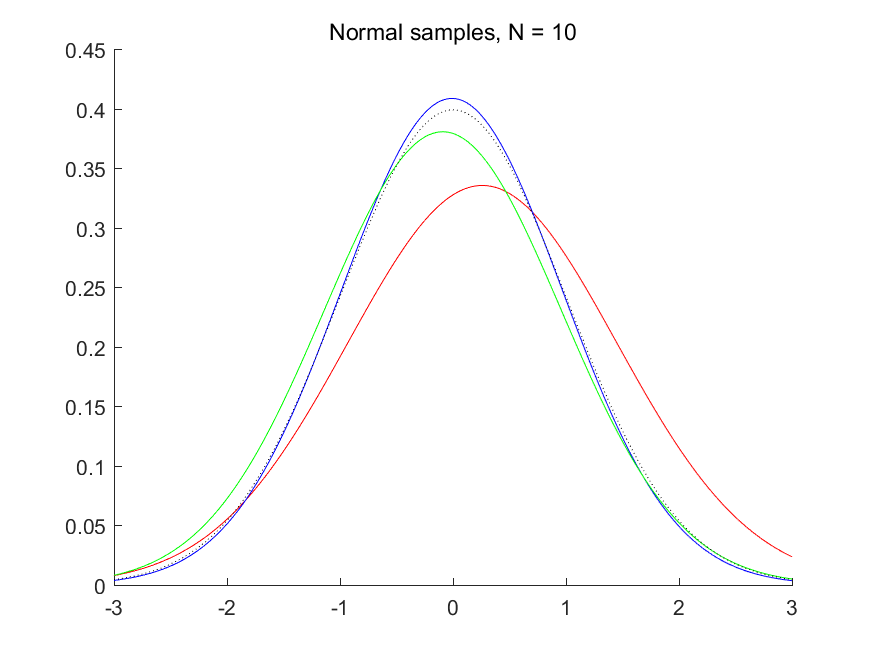
\includegraphics[width = 0.6\linewidth]{normal_10.png}
            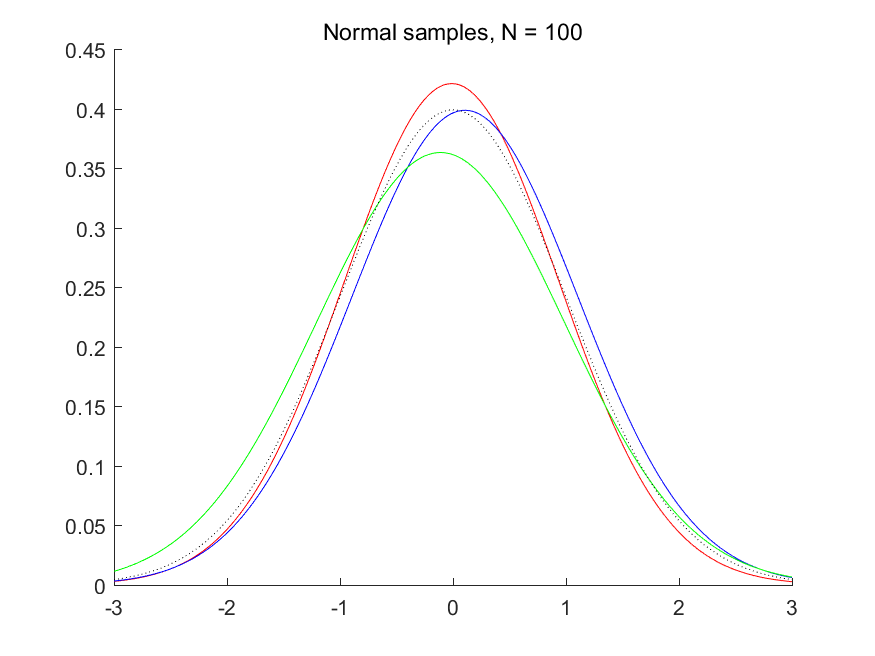
\includegraphics[width = 0.6\linewidth]{normal_100.png}
            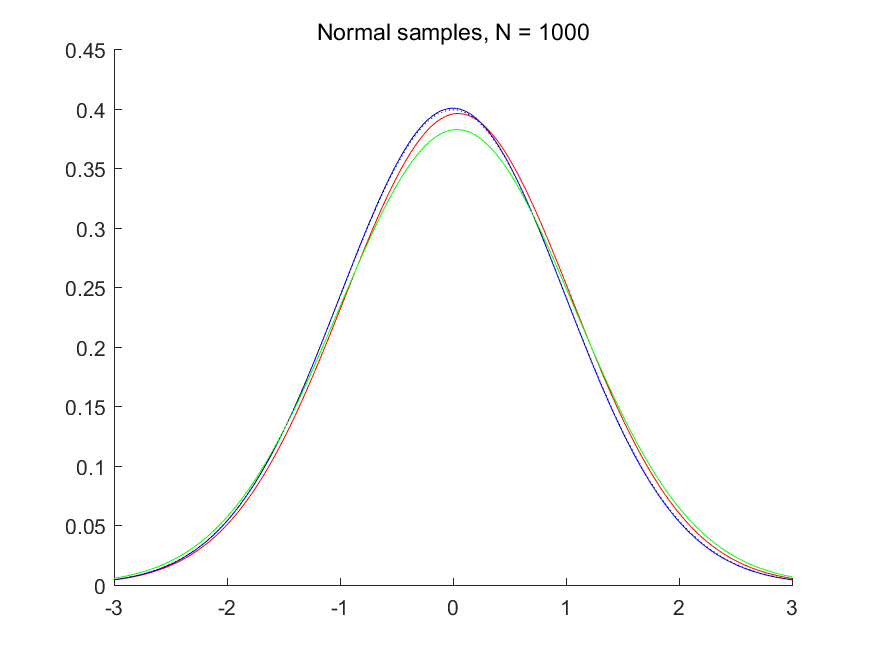
\includegraphics[width = 0.6\linewidth]{normal_1000.png}
            \caption{Density plots with estimated parameters for normal samples}
        \end{figure}
    }

    \subsection*{(4)}
    {
        Below are the density plot with estimated parameters for uniform samples:

        \begin{figure}[H]
            \centering
            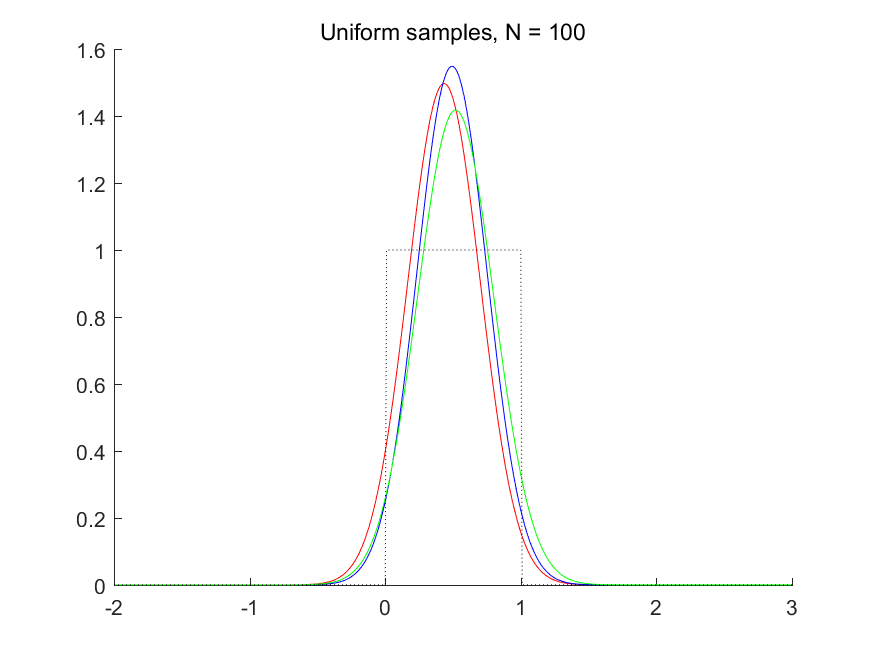
\includegraphics[width = 0.6\linewidth]{uniform_100.png}
            \caption{Density plot with estimated parameters for uniform samples}
        \end{figure}
    }

    \subsection*{(5)}
    {
        \begin{itemize}
            \item \textbf{Model selection} \quad A good prior model is essential to the MLE. The selected model should be of the distribution family that is similar to that of the data samples. By contrast, we see the normal model is not successful in subsection (4), where the sample is drawn from a distribution different from our normal model.

            \item \textbf{Sample size} \quad We find in subsection (3) that the larger the sample size, the more accurate the estimated distribution. From the Bayesian perspective, a larger sample size means more weight put on the observed data, than that on the prior knowledge. Although it is not exactly precise an interpretation here (as we do not have a prior distribution for the normal likelihood), it is obvious that more observations contribute to the model accuracy, if the model is reasonable.

        \end{itemize}
    }
}

\section*{Source Code}
{
    Please download the souece code from http://39.106.23.58/files/PR3\_2015011506.7z
}

\clearpage
\end{document}
    